\documentclass[11pt]{article}
\usepackage{color}
%\usepackage{fullpage} %!!!!! WARNING!!!! USE OF FULLPAGE PACKAGE LEADS TO COMPILATION ERROR WITH SIG-ALTERNATE
%\usepackage{mathptmx}
\usepackage{times}
\usepackage{subfig}
\usepackage{latexsym}
\usepackage{multirow}
\usepackage{mathtools}
\usepackage{epstopdf}

%\usepackage{amsmath, amssymb, amsfonts} %amsthm, }
\usepackage{graphics, graphicx, color}
%\usepackage[table]{xcolor}
%\usepackage{algorithm, algorithmic} %, ifthen}

%\usepackage{booktabs}
%\usepackage{caption}
%\renewcommand{\thesection}{\arabic{section}}

\usepackage{epsfig}
%\usepackage{amssymb}
%, amsthm}
%\usepackage{amsmath}
%\usepackage{amsfonts}

%\usepackage[ruled,linesnumbered]{algorithm2e}
\usepackage{hyperref}
%\renewcommand{\algorithmcfname}{ALGORITHM}
%\SetAlFnt{\small}
%\SetAlCapFnt{\small}
%\SetAlCapNameFnt{\small}
%\SetAlCapHSkip{0pt}
%\IncMargin{-\parindent}

%%
%\newtheorem{observation}{Observation}[section]
%\newtheorem{definition}{Definition}[section]
%\newtheorem{theorem}{Theorem}
%\newtheorem{lemma}{Lemma}[section]
%\newtheorem{claim}{Claim}[section]
%\newtheorem{example}{Example}[section]
%%\newtheorem{fact}{Fact}
%%\newtheorem{invariant}{Invariant}
%%\newtheorem{property}{Property}
%\newtheorem{corollary}{Corollary}
%\newtheorem{proposition}{Proposition}[section]

%\providecommand{\algorithmautorefname}{Algorithm}

\newcommand{\child}{{\tt\textsc{Child}}}
\newcommand{\In}{{\tt\textsc{In}}}
\newcommand{\Out}{{\tt\textsc{Out}}}

\newcommand{\suc}{{\tt\textsc{succ}}}
\newcommand{\pred}{{\tt\textsc{pred}}}

\newcommand{\attr}{{\tt{Att}}}

\newcommand{\oracle}{{\cal O}}



%
%\newcommand{\reva}[1]{#1}%{{\color{blue}{#1}{\typeout{#1}}}}
%\newcommand{\revb}[1]{#1}%{{\color{red}{#1}{\typeout{#1}}}}
%\newcommand{\revc}[1]{#1}%{{\color{magenta}{#1}{\typeout{#1}}}}
%
%%THE FOLLOWING IS TO WRITE THE REVIEWRS'S COMMENT, TO BE REPLACED BY {} LATER
%
%\newcommand{\revacomm}[1]{#1}%{{\color{blue}{\bf(#1)}{\typeout{#1}}}} %{}
%\newcommand{\revbcomm}[1]{#1}%{{\color{red}{\bf(#1)}{\typeout{#1}}}} % {}
%\newcommand{\revccomm}[1]{#1}%{{\color{magenta}{\bf(#1)}{\typeout{#1}}}} %{}

\newcommand{\reva}[1]{{\color{red} {#1}}}
\newcommand{\revb}[1]{{\color{blue} {#1}}}
\newcommand{\revc}[1]{{\color{magenta} {#1}}}

\newcommand{\scream}[1]{} %{{\color{purple}{\texttt{\textbf{ *#1*}}}{\typeout{#1}}}}
\newcommand{\blue}[1]{{\color{blue}{\bf * #1 *}{\typeout{#1}}}}
\newcommand{\red}[1]{{\color{red}{\texttt{\textbf{*#1*}}}{\typeout{#1}}}}
\newcommand{\ans}[1]{{\it ? #1 ?}{\typeout{#1}}}
\newcommand{\eat}[1]{}
\newcommand{\cut}[1]{}
\newcommand{\neweat}[1]{}
\newcommand{\eg}{\emph{e.g.}}
\newcommand{\ie}{\emph{i.e.}}
\newcommand{\figref}[1]{Fig.~\ref{#1}}
\newcommand{\angb}[1]{\langle #1 \rangle}
\newcommand{\comple}[1]{\widebar{#1}}


\newcommand{\photodb}{{\tt PhotoDB}} %{{\tt IndividualPhotoDB}}
\newcommand{\myphotodb}{{\tt MyPhotoDB}}
\newcommand{\cost}{{\tt cost}}
\newcommand{\pvt}{{\tt c}}

\newtheorem{observation}{Observation}
%\newtheorem{definition}{Definition}
%\newtheorem{theorem}{Theorem}
%\newtheorem{lemma}{Lemma}
%\newtheorem{claim}{Claim}
%\newtheorem{example}{Example}
%\newtheorem{fact}{Fact}
%\newtheorem{invariant}{Invariant}
%\newtheorem{property}{Property}
%\newtheorem{corollary}{Corollary}
%
%\newcommand{\ComputeSeparate}{\textsc{ComputeSeparate}}
\newcommand{\var}{\textsc{Var}}
\newcommand{\be}{\begin{enumerate}}
\newcommand{\ee}{\end{enumerate}}
\newcommand{\Algo}{\textsc{Algo}}
\newcommand{\No}{\textsc{No}}
\newcommand{\Yes}{\textsc{Yes}}
\newcommand{\Dom}{\texttt{Dom}}
\newcommand{\Codomain}{\texttt{CoDom}}
%\newcommand{\tup}[1]{\mathbf{#1}}
\newcommand{\tup}[1]{\vec{#1}}
\newcommand{\proj}[2]{\Pi_{{#1}}({#2})}

\newcommand{\true}{\textsc{True}}
\newcommand{\false}{\textsc{False}}

\newcommand{\Rows}{\texttt{Rows}}
\newcommand{\inset}{\texttt{P}}
\newcommand{\outset}{\texttt{Q}}

% For questions and answers.

\newcommand{\Tova}[1]{{\blue *(Tova): #1 *}}
\newcommand{\Benoit}[1]{{\purple *(Benoit): #1 *}}
\newcommand{\sudeepa}[1]{\red{*(Sudeepa): #1 *}}
%
%\newcommand{\scream}[1]{{\bf * #1 *}{\typeout{#1}}}
%\newcommand{\ans}[1]{{\it ? #1 ?}{\typeout{#1}}}
%\newcommand{\angb}[1]{{\langle #1 \rangle}{\typeout{#1}}}
%\newcommand{\eat}[1]{}
%\newcommand{\eg}{\emph{e.g.}}
%\newcommand{\ie}{\emph{i.e.}}


\newcommand{\wrt}{{with respect to~}}

\newcommand{\val}{{\texttt{val}}}
\newcommand{\type}{{\texttt{type}}}
\newcommand{\link}{{\texttt{link}}}
\newcommand{\for}{{\texttt{for}}}
\newcommand{\while}{{\texttt{while}}}
\newcommand{\repeatloop}{{\texttt{repeat\_loop}}}
\newcommand{\ismatch}{{\texttt{is\_match}}}


\newcommand{\select}{{\texttt{SELECT~}}}
\newcommand{\where}{{\texttt{WHERE~}}}
\newcommand{\from}{{\texttt{FROM~}}}
\newcommand{\groupby}{{\texttt{GROUP~BY~}}}
\newcommand{\orderby}{{\texttt{ORDER~BY~}}}
\newcommand{\desc}{{\texttt{DESC~}}}

\newcounter{countposid}
\setcounter{countposid}{0} 
\newcommand{\posid}{\addtocounter{countposid}{1}%
	\color{black!60}\small$\!_{\mathbf{\alph{countposid}}}$}
% guidelines at http://tab.computer.org/tcde/bull_author.html
\usepackage{deauthor,times,graphicx}
%\graphicspath{{authorname/}}

%\usepackage[dvipsnames,svgnames]{xcolor}
\usepackage{tikz}
\newcommand{\sky}{\ensuremath{\textrm{Sky}}}
\usepackage{amssymb, framed}
\usepackage{tikz}
\usepackage{rotating}
\usetikzlibrary{trees,shapes,snakes,patterns}
% % % --------------------------------------- % % %
% % % Macros to write comments for internal usage % % %
% % % --------------------------------------- % % %

\newcommand{\bcom}{\color{red!60}}
%\newcommand\bcom\iffalse
\newcommand{\ecom}{\color{black}}
%\let\ecom\fi
\begin{document}
%\title{Evaluating Preference Operators with Crowd\\ (a.k.a. Noisy Oracle)}
%\title{Evaluating Preference Operators with the Crowd\\ (modeled as a Noisy Oracle)}
\title{On Benchmarking for Crowdsourcing\\ and Future of Work Platforms}
%\title{Human-in-the-loop in the Era of Big Data and AI: Benchmarking the Future of Work\thanks{This work has been partially supported by ....}} % via Pairwise Comparisons}
\author{Ria Mae Borromeo\\
Philippines Open University\\
\texttt{{\footnotesize rhborromeo@up.edu.ph}}
\and
Lei Chen\\
HKUST\\
\texttt{{\footnotesize leichen@cse.ust.hk}}
\and
Abhishek Dubey\\
Vanderbilt University\\
\texttt{{\footnotesize abhishek.dubey@vanderbilt.edu}}
\and
Sudeepa Roy\\
Duke University\\
\texttt{{\footnotesize sudeepa@cs.duke.edu}}
\and
Saravanan Thirumuruganathan\\
QCRI, HBKU\\
\texttt{{\footnotesize sthirumuruganathan@hbku.edu.qa}}
}
\maketitle

% -------------------------------------------------------- %

%\red{need to discuss the title -- not much `crowd'}

\begin{abstract}
Online crowdsourcing platforms have proliferated over the last few years and cover a number of important domains, these platforms include from worker-task platforms such Amazon Mechanical Turk, worker-for-hire platforms such as TaskRabbit to specialized platforms with specific tasks such as ridesharing like Uber, Lyft, Ola etc.
An increasing proportion of human workforce will be employed by these platforms in the near future.
The crowdsourcing community has done yeoman's work in designing
effective algorithms for various key components, such as incentive design, task assignment and quality control. Given the increasing importance of these crowdsourcing platforms,
it is now time to design mechanisms so that it is easier to evaluate the effectiveness of these platforms. Specifically, we advocate developing benchmarks for crowdsourcing research.

Benchmarks often identify important issues for the community to focus and improve upon.
This has played a key role in the development of research domains as diverse as
databases and deep learning.
We believe that developing appropriate benchmarks for crowdsourcing will ignite further innovations.
However, crowdsourcing -- and future of work, in general -- is a very diverse field
that makes developing benchmarks much more challenging.
Substantial effort is needed that spans across developing benchmarks for
datasets, metrics, algorithms, platforms and so on.
In this article, we initiate some discussion into this important problem and
issue a call-to-arms for the community to work on this important initiative.
\end{abstract}

\section{Introduction}
\label{sec:intro}

Federated Learning (FL) is a distributed machine learning (ML) paradigm that trains a model across a number of participating entities holding local data samples.
% , without exchanging them. 
In this work, we focus on \emph{cross-device} FL that harnesses a large number (up to hundreds of millions) of edge devices with disparate characteristics such as availability, compute, memory, or connectivity
resources~\citep{kairouz2019advances}. %that harnesses potential
% Current applications of FL are designed to scale up to client populations of hundreds of millions or even billions. 
Two challenges to the success of cross-device FL are privacy and scalability. 
FL was originally motivated for improving privacy since data points remain on client devices. 
% and only small model updates were shared to a co-ordinating server.
However, as with other forms of ML, information about training data can be extracted via membership inference or reconstruction attacks on a trained model \citep{carlini2021membership,carlini2020extracting}, or leaked through local updates~\citep{MelisSCS19,geiping2020inverting}. 
Consequently, Secure Aggregation (\SecAgg) protocols were introduced to prevent the server from directly observing individual client updates, which is a major vector for information leakage~\citep{bonavitz2019federated,huba2021papaya}. 
Additional mitigations such as  Differential Privacy (DP) may be required to offer further protection 
against attacks~\citep{dwork2006calibrating,abadi2016deep}, as discussed in Section~\ref{sec:discussion}.
% , as discussed in Section~\ref{sec:discussion}.
%As an additional layer of protection against statistical inference attacks, SecAgg is usually paired with Differential Privacy (DP) \citep{dwork2006calibrating}. To realize the full promise of FL as a privacy-enhancing technology, we need both SecAgg and Differential Privacy.

Ensuring scalability to populations of heterogeneous clients is the second challenge for FL.
% There are many aspects for FL scalability, such as ensuring that model updates can be calculated efficiently 
% by devices with various capabilities and intermittent availability~\citep{bonavitz2019federated}.
% Here, we focus on the communication bottleneck as the primary concern.
Indeed, wall-clock training times are highly correlated with increasing model and batch sizes~\citep{huba2021papaya}, even with recent efforts such as FedBuff~\citep{nguyen2021federated},
% With increasing model and batch sizes, the wall-clock training time increases accordingly~\citep{huba2021papaya}. 
% Despite efforts such as buffered asynchronous aggregation~\cite{nguyen2021federated}, 
and communication overhead between the server and clients dominates model convergence time.
% cross-device FL remains bottlenecked by communication latency between the server and the clients. 
% \karthik{should we mention this paper in a different way? Fedbuff paper doesn't explicitly call out latency as an issue, nor do we run experiments to on async fl ourselves}  \ashkan{I also think the transition can be smoother: first we focus on scalability and billions. Then we say communication is the bottleneck} 
Consequently, compression techniques were used to reduce the communication bandwidth while maintaining model accuracy.
However, a fundamental problem has been largely overlooked in the literature: in their native form, standard compression methods such as scalar quantization and pruning are not compatible with \SecAgg. 
This makes it challenging to ensure both security and communication efficiency.
% at the same time.
% the default method to provide security for client update, 
% presenting an unpleasant dichotomy between security or efficiency. 


% Second, this is the most restricted direction, since upload bandwidth remains more restricted than download. 
% In the US, fixed-line broadband speeds typically achieve a ratio of $3\times$ to $20\times$ more download bandwidth than upload
% bottlenecks remain, and so we seek to reduce the message size of clients by \textit{compression}. 
% Compression has been widely proposed in various ML scenarios, in the form of pruning (removing model parameters) and quantization (reducing fidelity of parameter representation). 
% Indeed, these techniques have been successfully used in FL settings with appreciable improvements in communication while maintaining model accuracy. 
% However, there is a fundamental problem which has been largely overlooked in the literature: in their native form, these compression methods are not compatible with SecAgg, the default method to provide security for client updates. 
% This presents an unpleasant dichotomy: we can have security or efficiency, but not both. 
%
%
% In this paper, we resolve this gap by showing how to modify FL compression techniques to make them security-friendly. We focus on compressing \emph{uplink} updates from clients to the server for two reasons. 
% First, uplink communications are subject to Secure Aggregation protocols to ensure a high security bar, while downlink updates broadcasted by the server are deemed public. 
% Second, upload bandwidth is generally more restricted than download. For instance, according to the most recent FCC report, the ratio of download to upload speeds for DSL/cable providers\footnote{Fixed-line broadband is most relevant since FL is typically restricted to using unmetered connections, usually over Wi-Fi~\citep{huba2021papaya}.} in the US ranges between 3$\times$ to 20$\times$~\citep{fcc-broadband}.
% % This requires some meticulous changes to coordinate clients to use the same global (non-private) hyperparameters, and show that this coordination does not damage model quality. 
% % For the strongest compression methods, we step outside of the SecAgg primitive and propose a new secure primitive, Secure Indexing, which enables the best compression ratios without sacrificing utility. 
% Finally, efficient and secure uplink communication brings several benefits beyond speeding up convergence: 
% lowering communication cost reduces selection bias due to undersampling clients with limited connectivity, improving fairness and inclusivity metrics. 
% It also shrinks the carbon footprint of FL, whose fraction attributable to communication can reach 95\%~\citep{qiu2021first}.
%
%In this paper, w
We address this gap by adapting compression techniques to make them compatible with \SecAgg. We focus on compressing \emph{uplink} updates from clients to the server for three reasons. 
First, uplink communication is more sensitive and so is subject to a high security bar, whereas downlink updates broadcast by the server are deemed public. 
Second, upload bandwidth is generally more restricted than download bandwidth. For instance, according to 
a recent FCC report, 
%the most recent \modif{FCC\footnote{\modif{US Federal Communications Commission.}} report}, 
the ratio of download to upload speeds for DSL and cable providers\footnote{FL is typically restricted to using unmetered connections, usually over Wi-Fi~\citep{huba2021papaya}.} in the US ranges between 3$\times$ to~20$\times$~\citep{fcc-broadband}.
% Fixed-line broadband is most relevant since
% This requires some meticulous changes to coordinate clients to use the same global (non-private) hyperparameters, and show that this coordination does not damage model quality. 
% For the strongest compression methods, we step outside of the SecAgg primitive and propose a new secure primitive, Secure Indexing, which enables the best compression ratios without sacrificing utility. 
Efficient uplink communication brings several benefits beyond speeding up convergence: 
lowering communication cost reduces selection bias due to under-sampling clients with limited connectivity, improving fairness and inclusiveness. 
It shrinks the carbon footprint of FL, the fraction of which attributable to communication can reach 95\%~\citep{qiu2021first}.
In summary, we present the following contributions: 
\begin{itemize}
    \item We highlight the fundamental mismatch between two critical components of the FL stack: \SecAgg protocols and uplink compression mechanisms.
    
    \item We formulate solutions by imposing a linearity constraint on the decompression operator, as illustrated in Figure~\ref{fig:secagg_summary} in the case of TEE-based \SecAgg.
    
    \item We adapt the popular scalar quantization and (random) pruning compression methods for compatibility with the FL stack that require no changes to the \SecAgg protocol.
    
    \item For extreme uplink compression without compromising security, we propose Secure Indexing (\SecInd), a variant of \SecAgg that supports product quantization. %and admits a secure implementation.
\end{itemize}

\begin{figure*}[t]
    \centering
    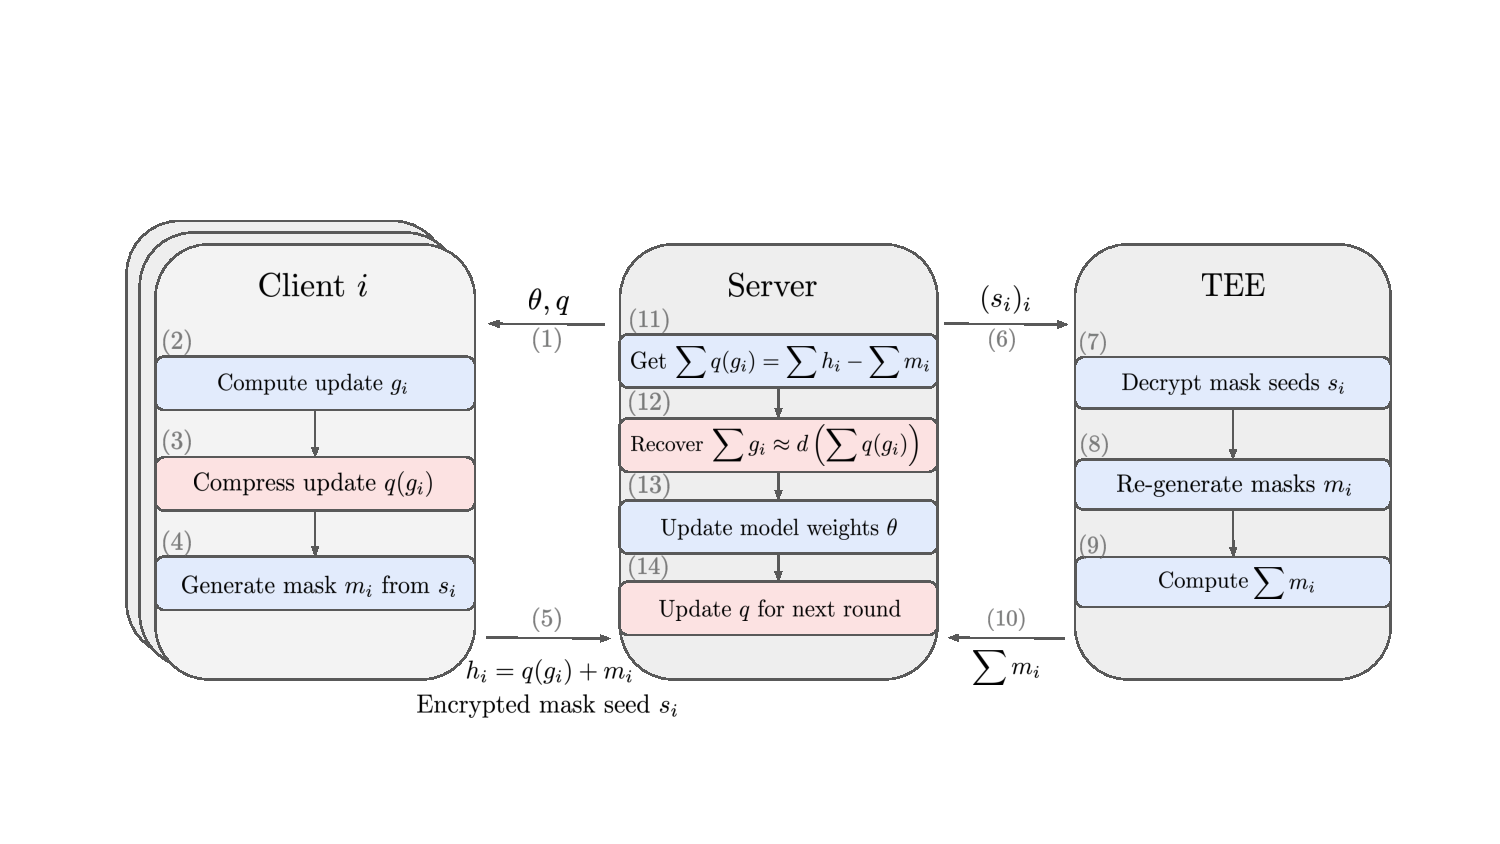
\includegraphics[width=0.8\textwidth]{figs/secagg_summary_new.pdf}
    %\vspace{-5mm}
    \caption{\label{fig:secagg_summary}
    Summary of the proposed approach for one FL round, where we omit the round dependency and \modif{Differential Privacy (DP)} for clarity. Blue boxes denote standard steps and red boxes denote additional steps for uplink compression. Client $i$ computes local model update $g_i$, compresses it with the compression operator $q$, and encrypts it by adding a random mask $m_i$ in the compressed domain, hence reducing the uplink bandwidth (steps 2--4). The server recovers the aggregate in the compressed domain by leveraging any \SecAgg protocol \modif{(steps 7--13, with a TEE-based \SecAgg, see Section~\ref{subsec:secagg})}. Since the decompression operator $d$ is linear, the server can convert the aggregate back to the non-compressed domain, up to compression error (step 12). As with the model weights $\theta$, the compression operator $q$ are also periodically updated and broadcast by the server (step 14). 
    In Section~\ref{sec:method}, we apply the proposed method to scalar quantization and pruning without impacting \SecAgg and propose Secure Indexing, a variant of \SecAgg for extreme uplink compression with product quantization. See Section~\ref{subsec:secagg} for details about \SecAgg and Section~\ref{sec:discussion} for a discussion on~DP.
    }
    \vspace{-3mm}
\end{figure*}



% Our focus in this paper is on 

%Second, scaling cross-device (synchronous) FL to millions of clients with various capabilities and intermittent availability \citep{bonavitz2019federated} suffers from diminishing returns: the wall-clock training time plateaus as the number of clients keeps increasing~\citep{huba2021papaya}. Even though this challenge can be addressed by leveraging the buffered asynchronous aggregation technique proposed by \cite{nguyen2021federated}, compatible with DP and SecAgg, the asynchronous protocol remains bottlenecked by communication latency between the server and the clients.


%Considering the above privacy and scalability goals, we focus on enabling efficient FL communications while keeping a high privacy bar. In addition to the primary objective of speeding up convergence, reducing communication costs brings other significant benefits. Lowering communication requirements addresses selection bias due to undersampling clients with limited connectivity, improving fairness and inclusivity metrics. Better communication efficiency shrinks the carbon footprint of FL, whose fraction attributable to communication can reach 95\%~\citep{qiu2021first}. %Finally, training larger model in FL would be a possibility, when the communication cost is reduced, because local memory or compute requirements can be addressed by modifying the local training loop, for instance with gradient checkpointing \citep{chen2016training}. However, some form of compression would be required to enable efficient communication.


%First, compressing model updates from the client to the server presents several challenges due to compatibility with SecAgg and is an area suitable for further research. 
%Second, upload bandwidth is generally more restricted than download. For instance, according to the most recent FCC report, the ratio of download to upload speeds for DSL/cable providers in the US ranges between 3$\times$ to 20$\times$~\citep{fcc-broadband}. We consider broadband speeds here because devices participate in the FL training while connected to fixed broadband, usually through Wi-Fi~\citep{huba2021papaya}.




% Hence, FL provides the ability to leverage data from massive client populations while ensuring the security and privacy of the client data.
% Go further: compatibility with DP / compression as a mitigation techniques of attacks
% Model and gradient compression intrinsically different.
%  Why not having the secure enclave perform the aggregation?
\section{Benchmarking Metrics}
\label{sec:benchmarkingMetrics}

As mentioned before, the diversity of the tasks and the presence of multiple stakeholders
makes the process of designing a comprehensive set of metrics very challenging.
In this section, we make an initial attempt in identifying a set of relevant metrics
that are relevant for FoW research.

\textbf{Desiderata for FoW Metrics.}
Metrics are the primary mechanism by which the performance of an FoW platform is evaluated.
Crowdsourcing has been used in a number of diverse domains -- so the metrics must be both generic and comprehensive.
Currently, most of the metrics are focused on the requestors.
It is important to design metrics that take into account the needs of all three major stakeholders -- workers, requestors and platforms.
It should be able to handle both quantitative (such as computational criteria)
and qualitative aspects (such as human and social factors).

\subsection{Metrics for FoW Platforms}
We begin by describing few metrics that could be used to quantify any given FoW platforms.

\textbf{Crowd Size, Diversity and Rate of Participation.}
Workers are an indispensable part of any FoW platform.
So one of the most basic metrics for the platform measures the size of the crowd.
Typically, requestors would prefer a platform with more workers as it gives a wider pool for recruitment.
Of course, size only gives an incomplete perspective of the platform.
The diversity of the crowd is often a better indicator of the quality of worker pool
especially for knowledge intensive crowdsourcing tasks.
A diverse crowd with different background and perspectives
often results in more creative solutions.
Finally, one metric that is useful to measure how thriving a platform is
participation rate that measures the number of workers who are active and perform tasks in a given unit of time such as  a week or a month.
In a thriving FoW platform, one would expect that this number will be large.
An alternate metric could measure the average amount of time that is spent by workers on the platform.

\textbf{Worker Skill Distribution.}
Another key aspect of the FoW platform is the skill distribution of the workers.
In a generic FoW platform such as AMT, each worker and task could be annotated with a set of skills
such as translation, writing, comprehension and so on.
Ideally, requestors would prefer a platform with workers having diverse skills.
Another key aspect is the alignment between the skill distribution
available in the worker pool and the distribution required by the task pool.
Such a misalignment often results in the frustration of both workers and requestors.

\textbf{Task Diversity and Complexity.}
Similarly, it is important to measure the distribution of the tasks themselves.
It is important for the platform to have a wide variety of tasks involving different skills
and varying complexity ranging from easy to difficult.
A steady stream of monotonous or complex tasks could reduce worker motivation and result in turnover.

\textbf{Efficiency Metrics: Tail Latency and Throughput.}
The FoW platform could have a number of quantitative metrics that measure its performance.
Two of the key metrics are latency and throughput.
Latency measures the time taken between posting of a job and its completion.
Of course, some latency is inevitable due to the inherent nature of humans.
However, a large latency would preclude certain tasks that require interactive responses from being posted on the platform.
In addition to the mean and median latencies, it is also important to measure
the tail latencies corresponding to the 95-th or 99-th percentile of task latencies.
Similarly, it is also important to measure throughput which could measure
the number of tasks completed in any given unit of time.
Throughput could also be used to evaluate specific algorithms such as task assignment
wherein it measures the number of tasks for which workers were matched with.

\textbf{Reliability and Robustness to Adversaries.}
Any major FoW platform attracts a wide variety of adversaries
such as workers who are scammers out to make a quick buck by possibly colluding with other workers.
This could also include requestors who either maliciously reject tasks completed by workers so as to not pay them or those who use crowdsourcing for illegal or unethical purposes.
It is important that the platform has sufficient mechanisms so that it is robust against such adversaries.
Crowdsourcing is increasingly being used for major tasks and it is important that the platform is reliable and does not crash.

\textbf{Usability of the FoW Platform Interface.}
An under-appreciated aspect of FoW platforms is how user friendly the interface is.
This is applicable to both the workers and requesters.
Any large FoW platform attracts a diverse group of requestors and workers
who may not be fluent in how the platform works.
For example, the requestors could be domain scientists such as psychologists or social scientists
with limited knowledge of computer science.
Similarly, workers could have a wide variety of educational levels.
Hence, it is important that the platform's interface is intuitive and allows both requestors and workers to complete the tasks efficiently.

\subsection{Metrics for FoW Workers}
Workers are a key part of the platform and its success hinges on learning appropriate information about the workers and use it effectively so that all the stakeholders are satisfied.
We enumerate below a number of key facets of human workers that must be systematized and measured.
Such metrics have the potential to represent the worker holistically than the current approach of quantifying the worker simply as a number based on the task approval rate.

\textbf{Human Factors.}
It is important to model the behavior or characteristics of human workers in any crowdsourcing platform.
This has a number of applications such as assigning appropriate workers to tasks to ensure their completion
and recommending appropriate tasks to workers to increase job satisfaction.
Prior work~\cite{amer2016human,roy2013crowds,cullina2015measuring}
typically involve identifying appropriate human factors,
integrating them into FoW components such as task assignment and
estimating them from past interactions with FoW platforms.
For the reminder of the section, we discuss the major human factors.
Systematically formalizing them and integrating them holistically into FoW platforms is a major open challenge.

\textbf{Skill, Knowledge and Expertise.}
Most generic crowdsourcing platforms such as AMT could have a set of domains
$D=\{d_1, d_2, \ldots, d_m\}$ that denote the various knowledge topics.
Consider a task of translating documents from English to French.
Even this task requires multiple skills such as comprehension of English language,
writing and editing in French.
Generic platforms have a wide variety of task types with large platforms such as Crowdworks
supporting as much as 200 types of tasks.
Given this setting, it is important to enumerate the set of skills needed by the tasks
and possessed by the workers.
One could quantify the skill using categorical values (not knowledgeable, novice, knowledgeable and expert)
or in a continuous $[0, 1]$ scale.
So, a value of $0$ for a specific skill such as English comprehension denotes no expertise
while the value of $1$ could denote complete mastery.

\textbf{Worker Motivation.}
This is one of the most important human factors and a key component of the worker to be measured.
Understanding worker motivations could be used to improve the performance of the FoW platform
through a more informed matching of workers with tasks.
However, understanding what motivates workers is not so obvious.
Some workers could be motivated by monetary compensation while others are motivated by fun and enjoyment.
It has been found that prior work social studies on
workplace motivation is also applicable to FoW platforms~\cite{kaufmann2011more,pilz2013does}.
In fact, there are as many as 13 factors that are highly relevant for worker motivation~\cite{kaufmann2011more}.
These could be categorized as intrinsic and extrinsic motivation.

Intrinsic motivation include aspects of tasks such as~\cite{kaufmann2011more}
skill variety (preference for tasks requiring a diverse collection of skills),
task identity (the worker perception about the completeness of the task),
task autonomy (the degree of freedom allowed during the task),
feedback during the task completion and so on.
Extrinsic motivation includes monetary compensation, human capital advancement and
signaling (performing a task to give a strategic signal to environment).

\textbf{Metrics for Group based Human Factors.}
The increasing popularity of knowledge intensive crowdsourcing tasks requires collaboration.
Hence, it is important to measure the various factors that are relevant to modeling worker collaboration.
The most important of those is worker-worker affinity that measures the collaborative effectiveness of any two workers. This could be extended to measure the social cohesiveness of any group of workers.
It is often desirable to form a group of workers where the aggregate pairwise affinity is large.
Of course, there is a natural diminishing returns when increasing the group size beyond certain threshold dubbed critical mass.


\subsection{Metrics for FoW Tasks}
Tasks (and requestors) form the final leg of FoW platforms.
A number of metrics described for platforms are also applicable for tasks.

\textbf{Accuracy and Quality.}
This is often the most important metric for the requestors.
If the responses of the workers are accurate, then most popular approaches for
aggregating worker responses will provide accurate results.
It is important for the requestor that the completed crowdsourcing tasks have a high accuracy rate.

\textbf{Cost.}
The requestor often wants to complete a given task with high accuracy while minimizing the monetary payment or the worker effort.
There has been extensive work on identifying appropriate workers while satisfying the quality and cost constraints of the tasks.
The requestor has a natural cost-benefit tradeoff and higher cost often deters them without the requisite quality.

\textbf{Completion Rate and Latency.}
The human workers create an uncertainty in terms of task completion.
It is possible that a worker accepts a task but does not complete it immediately.
This creates a straggler effect where some workers could delay the completion of the tasks.
This is especially important for longer tasks where workers losing motivation is a key risk factor.
This affects the requestor in two ways.
First, any task consist of a number of micro-tasks all of which need not be completed.
Higher the completion rate, the better it is for the requestor.
Second, for complex tasks that often have a binary outcome (task completed or not),
it could dramatically increase the latency.
Having systematic method to measure these two phenomenon is quite important.

\textbf{Fairness Related Metrics.}
There has been intensive research on how to quantify fairness.
In our context, it is important to ensure that the platform and the task requestor are seen as fair.
For example, workers who did similar tasks should be paid similar compensation.
Similarly, the worker submissions must not be rejected without a valid reason and so on.

\section{Benchmarking Data}
\label{sec:benchmarkingData}
With the proposed metrics, the next task is to design Benchmarking data to test the effectiveness of the FoW  platforms. Existing works \cite{yongxin2016online, ChengCY19, ChenCZC19} often use real data set to test. However, it is hard if it is not impossible to derive statistic information of real data. Without knowing the characteristic of real data, it will be difficult to choose the right real data to test. Moreover, even we use all the real data sets, we still do not know if we have tested all the possible worst case scenarios, the robustness of the platform is still unknown. Thus, in this section, we mainly discuss how to design synthetic benchmarking data of workers and tasks to test the FoW platforms.

\subsection{Benchmarking data for workers}

There are many factors we should consider to design benchmarking data of workers, which are listed as follows.

\textbf{Worker's expertise. } 
As we can observe from a crowdsourcing platform, given the same question/task,  different workers may offer different answers. This is because different workers often have different level of expertise in different domains. Thus, when we design benchmarking data of workers, we should assign  workers into different categories (domains) with different expertise levels. Moreover, different category and expertise level distributions should be generated.

\textbf{Worker's preference. } 
Worker's preferences towards different types of tasks also determine the workers' willingness to accept the tasks. For example, some workers prefer image labelling tasks to language translation tasks,  if both types of tasks are available in the platform, with a very high probability, they will choose the image labeling tasks. Thus, benchmarking data of workers should take worker's preferences (categories of tasks) into consideration. Again, we should generate different distributions for category preference of workers.

\textbf{Worker's activeness. } 
Given the same crowdsourcing platform, some workers are quite active and solve many tasks/question within a short period of time, while some only solve a few questions but spend quite long time. Therefore, to generate benchmarking data of workers, we can use  the number of tasks completed with a specified period time as the activeness factor and simulate it with different distributions.


\subsection{Benchmarking data for tasks}

Similar as workers, for tasks, we also need to consider different factors when we want to generate benchmarking tasks.

\textbf{Task's category and difficulty. } Given a crowdsouring platform, there are many different types of tasks. For the same type of tasks, the difficulties are also different. For example, given an image, an image classification task is much easier compared to an object identification task.  Therefore, we need to consider categories and difficulty levels to generate tasks with different distributions.

\textbf{Task's budget. }  Given the same tasks with different budgets,  the task with a higher budget is often accepted much faster than the one with a lower budget. Of course, this does not indicate that tasks with higher budget will get higher quality answers.  We need to generate budgets with different distributions for the tasks.

\textbf{Task's completion time. } When the requester posts a task on the crowdsourcing platform, she often sets up a completion time, which is the time that the requester expects the answer back. Depends on the urgency of the tasks,  different tasks often have different specified completion time. We need to generate completion time with different distributions for the tasks.

\textbf{Tasks' required number of answers. } For some tasks, the requester only needs one answer, such as simple true/false questions, while for complicated tasks, such as object identification, more workers are needed to verify the correctness of labelled objects.  Thus, we need to take tasks' required number of workers as another factor to generate task data.

%%\section{Benchmarking FoW Implementations}
%While metrics is a fundamental aspect of benchmarking,
%there are a number of other dimensions that are equally important.
%In this section, we highling some of them.

%\textbf{Benchmarking Datasets.}
%Crowdsourcing is often considered as an inexpensive mechanism to obtain benchmark datasets.
%Popular datasets for challenging AI tasks such as computer vision and natural language processing
%were obtained through crowdsourcing.
%This allows the requestors to capture human knowledge and intuition
%that is then used to train ML models.
%Hence, it is quite ironic that there is a lack of benchmark datasets for evaluating crowdsourcing research.
%This is a major stumbling blocks in algorithmic research on crowdsourcing.

%FoW platforms have a number of components such as
%task assignment, truth inference from worker responses, estimating human factors and so on.
%Developing benchmarks are often beneficial for both platforms and requestors.
%Not surprisingly, major platforms such as Figure Eight have open sourced a large collection of (small-ish) tasks and their responses~\cite{Figure8DataForEveryone}.
%Similarly, there are some early efforts for obtaining multiple (small) datasets for evaluating algorithms for truth inference~\cite{zheng2017truth}.
%While promising, these are often insufficient.
%It is often desirable to have a single comprehensive dataset that is diverse, large, realistic and has a good mix of easy and challenging tasks.

%\section{Concluding Remarks}
\label{sec:discussion}
In this paper, we reconcile efficiency and security for uplink communication in Federated Learning. 
We propose to adapt existing compression mechanisms such as scalar quantization and pruning to the secure aggregation protocol by imposing a linearity constraint on the decompression operator. 
Our experiments demonstrate that we can adapt both quantization and pruning mechanisms to obtain a high degree of uplink compression with minimal degradation in performance and higher security guarantees. For achieving the highest rates of compression, we introduce \SecInd, a variant of \SecAgg well-suited for TEE-based implementation that supports product quantization while maintaining a high security bar. 
%We plan to extend our work to other federated learning scenarios, such as asynchronous FL, and further investigate the interaction of compression and privacy.
%\section{Extensions} 
As mentioned in Section~\ref{sec:intro}, we {may want } both \SecAgg and Differential Privacy~\citep{abadi2016deep} to realize the full promise of FL as a privacy-enhancing technology. 
While our primary focus is on enabling efficient and secure uplink communication, we emphasize that the proposed approaches are compatible with user-level DP. 
For instance, {at the cost of increasing the complexity of the trusted computing base}, DP noise can be added natively by the TEE with our modified random pruning or scalar quantization approaches. 
For PQ  and \SecInd, {we can have the TEE to add noise in the assignment space (\ie outputting a noisy histogram), or to map the histogram to the codeword space and add noise there.
Each option offers a different tradeoff between privacy, trust, and accuracy; we leave detailed evaluation to future work.}




%\modif{\textbf{Compatibility with DP.} 
%\sout{it would require, however, to transfer the aggregation to TEE or to design a DP mechanism in the assignment space, since DP noise must be added by the TEE and not by the server.}}

%\modif{\textbf{Efficiency and Privacy.}} A separate line of work {aims} to combine communication efficiency and privacy. 
%For instance, \cite{triastcyn2021dprec} develop a method that unifies compressed communication and DP (where integration with \SecAgg is left as an open problem), while \cite{chaudhuri2022privacyaware} design a privacy-aware scalar compression mechanism within the \emph{local} differential privacy model.

%\graham{\sout{
%\modif{\textbf{Broader Social Impact. }} In this work, we propose to enhance the privacy of individuals who may contribute to training ML models and simultaneously enable more individuals to participate in private training, who might otherwise have been excluded due to resource constraints. }}
% Indeed, Federated Learning could enable a malicious server to access individual model updates that can leak personal information. Hence, we propose a secure way to communicate the individual model updates.

% - Generic and less data-dependent codebook
% - Model compression 
% - Compression and DP
% - Error correction

% There are multiple extensions of PQ, such as having multiple codebooks per matrix  (which increases the cost of storing the codebooks) or performing the assignments with other norms than the $L_2$ norm.



% As a side note, \cite{jia2022federated} propose to perform domain adaptation by fine-tuning a small fraction of the model parameters, which is naturally compatible with Secure Aggregation, but requires to start from a pretrained model. 

\section{Research Directions}\label{sec:research}

Creating a comprehensive benchmark for online job platforms with complex interactions among human workers and requesters, machines, and AI agents is a non-trivial task. Here we list some challenges that need to be addressed when we design such a benchmark.


\textbf{Broad applicability for use in academia and industry.} The benchmarks designed for evaluating the platforms should be able to cover  different types of works, platforms, and workers.  Real applications have different requirements, especially for many real industry applications, therefore, developing a ``leaderboard benchmark'' with single dataset and single application may not work. Instead, we need to support tailored benchmarks for different workloads and have sufficient diversity in the requirements within the benchmark to  satisfy the needs of different platforms, especially from industry (e.g., as done in TPC benchmarks used to evaluate performances of query evaluation supporting different workloads).

\textbf{Acceptability in Research Communities.} One practical challenge after designing a benchmark is to getting the benchmark widely  accepted in the research community and industry. This would need wider discussions and involvement  of all the relevant players like the crowdsourcing platforms from industry  and academia, research communities, and also possibly the workers and requesters who use these platforms.
%(SAT  solver, diversity, coverage of jobs, domain specific)


\textbf{Incorporating Metrics capturing human factors that are not easy to measure.}
One can be seen that a number of metrics like latency, throughput, or cost are easy to measure (although can be measured in multiple ways). On the other hand, some metrics, especially the ones related to human factors such as fairness, equity, and satisfaction, are difficult to measure. Incorporating ideas from the recent advances in research on  fairness and ethics from data management, ML/AI, and also non-computational domains like psychology, cognitive science, sociology, laws, and policy would be useful.

\textbf{Handling multiple criteria and optimizations:} Satisfying multiple metrics all at the same time may lead to multi-objective optimization problems, which are typically computationally intractable. As in computational challenges, formulating the problems meaningfully, designing efficient approximation algorithms with formal guarantees, and also developing efficient tools that produce good results in practice will be required. On the other hand, one can explore whether keeping all the criteria separate and giving individual scores to those criteria work better.

\textbf{Supporting interactions with AI agents:} Since AI agents are used in different stages in an online job platform, we need to develop benchmarks that enable comparison of effectiveness and interactions of AI agents and humans on jobs of various categories. Such a benchmark will have to continuously updated as AI technology improves.

\textbf{Measuring robustness:} Measurement of robustness of the platform or of the matching algorithm used in the platform would require creation of adversarial benchmarks that will enable assessment of effectiveness of integrity checks and anomaly detection mechanisms built into the platforms. For instance, if an adversarial requester attempts to ruin the reputation of a worker with poor ratings, or if a worker attempts to game a system by providing wrong inputs, a good platform would be able to detect or defect such attempts by using other information collected in the process, which might be one of the desired properties of the benchmark.

\textbf{Reproducibility:} Results that use standard benchmarks used in different contexts (e.g., TPC-H or TPC-DS data for evaluating scalability in data management) are repeatable or reproducible. On the other hand, tests involving humans are not always repeatable benchmark tests results could vary for every test run. Allowing some level of differences in the results and considering mean/variances might be needed while developing the benchmarks.

\textbf{Synthetic benchmark data generation:} Based on the data distribution of data logs, such as availability of workers/jobs and dynamics of the platform, collected from real job markets, how can  we generate synthetic  benchmark data which follows the same data distribution under the similar environment scenarios to test various aspects of users, jobs and platforms, such as effectiveness and scalability.

%!TEX root = ../main.tex

\section{Concluding Remarks}
\label{conclusion}

There exist many systems for monitoring and analyzing spatio-temporal data, such as a dashboard for visually tracking the outbreak of COVID-19~\cite{dong2020interactive} and a tweet stream sentiment analysis system for US election 2016~\cite{DBLP:conf/kdd/PaulLTYF17}. 
One lesson from the existing systems is  that they are usually designed on a case-by-case basis and built from scratch, which cannot fully leverage the recent techniques for data integration and automatic visualization.

On the one side, \sys-COVID-19 shares many common visualizations as the other popular websites for tracking COVID-19 cases.
On the other side, it differs from the others in 
(1) \sys-COVID-19 is based on a general end-to-end framework \sys, and leverages recent techniques for data preparation (\eg~{\sc VisClean}~\cite{visclean-icde}) and for visualization recommendation (\eg~{\sc DeepEye}~\cite{deepeyeicde});
%
(2) it supports linked visualization for the users to easily zoom in/out multiple visualizations by a single click; and
%
(3) it also obtains some private data that is not publicly available, so it can demonstrate some unique features.
%
%Hopefully we can survive the war of fighting COVID-19 with the minimum cost, and by the time of VLDB 2020, we will have much more to demonstrate.

%\add{Open Challenges: (1) Smart and Effective Data Preparation. (2) Data Sharing Platform. (3) Intelligent Data Analysis (4) Abstract general modules, the system supports reusability}

%GiG




\bibliographystyle{abbrv}
\bibliography{crowd}
\end{document}
